
This section explains the technical background behind Paper II, see \autoref{chapter:hospital}. This study investigates the potential advantages of using a modern machine-learning model compared to classical logistic regression to predict the risk of patients being re-hospitalized after fast-track hip and knee replacements. In particular, the patients were grouped into two groups. The first group were the so-called ``risk-patients'' that stayed at least 4 days in the hospital post surgery or were re-hospitalized within 90 days of surgery. The second group were the non-risk-patients. As such, this is a binary classification problem where the patient's risk-score is predicted based on historical data. The machine learning models were trained on 33 variables, of which 7 were continuous, related to the patient's medical record, such as age, gender, the use of walking aid, anaemia, diabetes, etc. A total of 22.017 patients were included in the study, of which 1.476 were risk-patients.


Most classification and regression problems fall under the same machine learning (ML) branch called supervised learning. In supervised learning, the goal is to find the hypothesis $h^*$ in the hypothesis set $\mathcal{H}$ that matches the unknown, ``true'' data-generating function $f: \mathcal{X} \rightarrow \mathcal{Y}$ optimally, where $\mathcal{X}$ is the input space and $\mathcal{Y}$ is the output space. Assuming that we have access to realizations of $f$, the so-called training data $\mathcal{D}_\mathrm{train} = \{(\mathbf{x}_i, y_i)\}_{i=1}^N$, we can use a learning algorithm $\mathcal{A}$ combined with the training data to estimate $h^*$ \autocite{abu-mostafaLearningData2012a}. Here $N$ refers to the number of training samples and $\mathbf{x}_i$ is the $i$th observation with the true label $y_i$. This process is illustrated in \autoref{fig:ML-setup}.

\begin{figure}[htbp]
    \sidecaption{
        Illustration of how to learn from data in a supervised learning setting. Adapted from \autocite{abu-mostafaLearningData2012a}.
        \label{fig:ML-setup}}
    \centering
    \includegraphics[width=0.9\textwidth]{figures/illustrator/ML-learning.pdf}
\end{figure}

Both logistic regression (LR) and ML models can be viewed through the lens of \autoref{fig:ML-setup}, just with $|\mathcal{H}_\mathrm{LR}| \ll |\mathcal{H}_\mathrm{ML}|$, i.e. the machine learning model is a lot more complex than the logistic regression model and the hypothesis space thus significantly larger. While sufficiently parameterized ML methods can in theory achieve perfect performance on the labelled training set, one is rarely interested in the predictive power of $h^*$ on the training set, as the truth is already known. Instead, one often wish to apply the trained model to new, unseen data where the truth is unknown.

Assessing the performance of $h^*$ on unlabelled data can be difficult. A naive estimate would be to assume that the performance on new, unseen data is the same as on the training data. However, this would likely be a poor estimate due to overfitting and thus bias the predicted performance, especially for high cardinality hypothesis sets. \autocite{abu-mostafaLearningData2012a}. The concept of overfitting is illustrated in \autoref{fig:ML-overfitting}, which shows the training loss as a function of model complexity. The figure shows how more advanced models can achieve lower and lower training losses, however, at some point they start to overfit, leading to higher validation losses. The validation loss is the error on unseen data and is thus the quantity of interest. The goal is to find the sweet spot between underfitting and overfitting.

\begin{figure}[htbp]
    \sidecaption{
        Illustration of the loss as a function of model complexity. The training error is shown in blue and validation error in red. Figure from \cite{michelsenPhysicistApproachMachine2020}.
        \label{fig:ML-overfitting}}
    \centering
    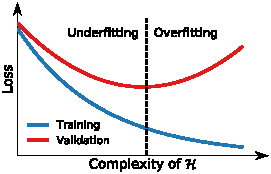
\includegraphics[width=0.6\textwidth]{figures/MasterThesis-overfitting.pdf}
\end{figure}

To avoid overfitting and get accurate estimates of the performance of $h^*$, we use a technique called cross-validation (CV). In the simplest way, this can be done by splitting the data into two sets, one called the training and one called the validation set, and then only train on the training set. Afterwards the trained model can be evaluated on the validation set without biasing the performance estimate. This process can further be refined by splitting the data into $K$ folds and then repeating the process $K$ times, where each fold is used as the validation set once.
This is called $K$-fold cross-validation and is illustrated in \autoref{fig:ML-crossval-kfold} \autocite{murphyMachineLearningProbabilistic2012,hastieElementsStatisticalLearning2016}.
$K$-fold cross validation works well in many cases, yet in the case of temporal data, it also risks introducing bias in the performance estimates, since, in the different folds, it, effectively, is allowed to ``look into the future''. The most extreme case of this is shown in the bottom of \autoref{fig:ML-crossval-kfold} where the model trains on future data and is then evaluated on past data (relative to test fold). In many time dependent datasets, such as the one in Paper II, this is undesirable. Instead, we use a technique called temporal cross validation, see \autoref{fig:ML-crossval-temporal}, which circumvents this problem by only allowing the model to train on past data and evaluate on future data \autocite{tashmanOutofsampleTestsForecasting2000a}. As the patient data is time dependent, this is the technique we use in Paper II.
% The fraction of rehospitalizations decreased over time due to surgerilogical improvements.

\begin{figure}[htbp]
    \centering
    \sidecaption{
        Two types of cross validation: $K$-fold cross validation, and temporal cross validation. Both figures from \cite{michelsenPhysicistApproachMachine2020}.
        \label{fig:ML-crossval}}
    \begin{subfigure}{.5\textwidth}
        \centering
        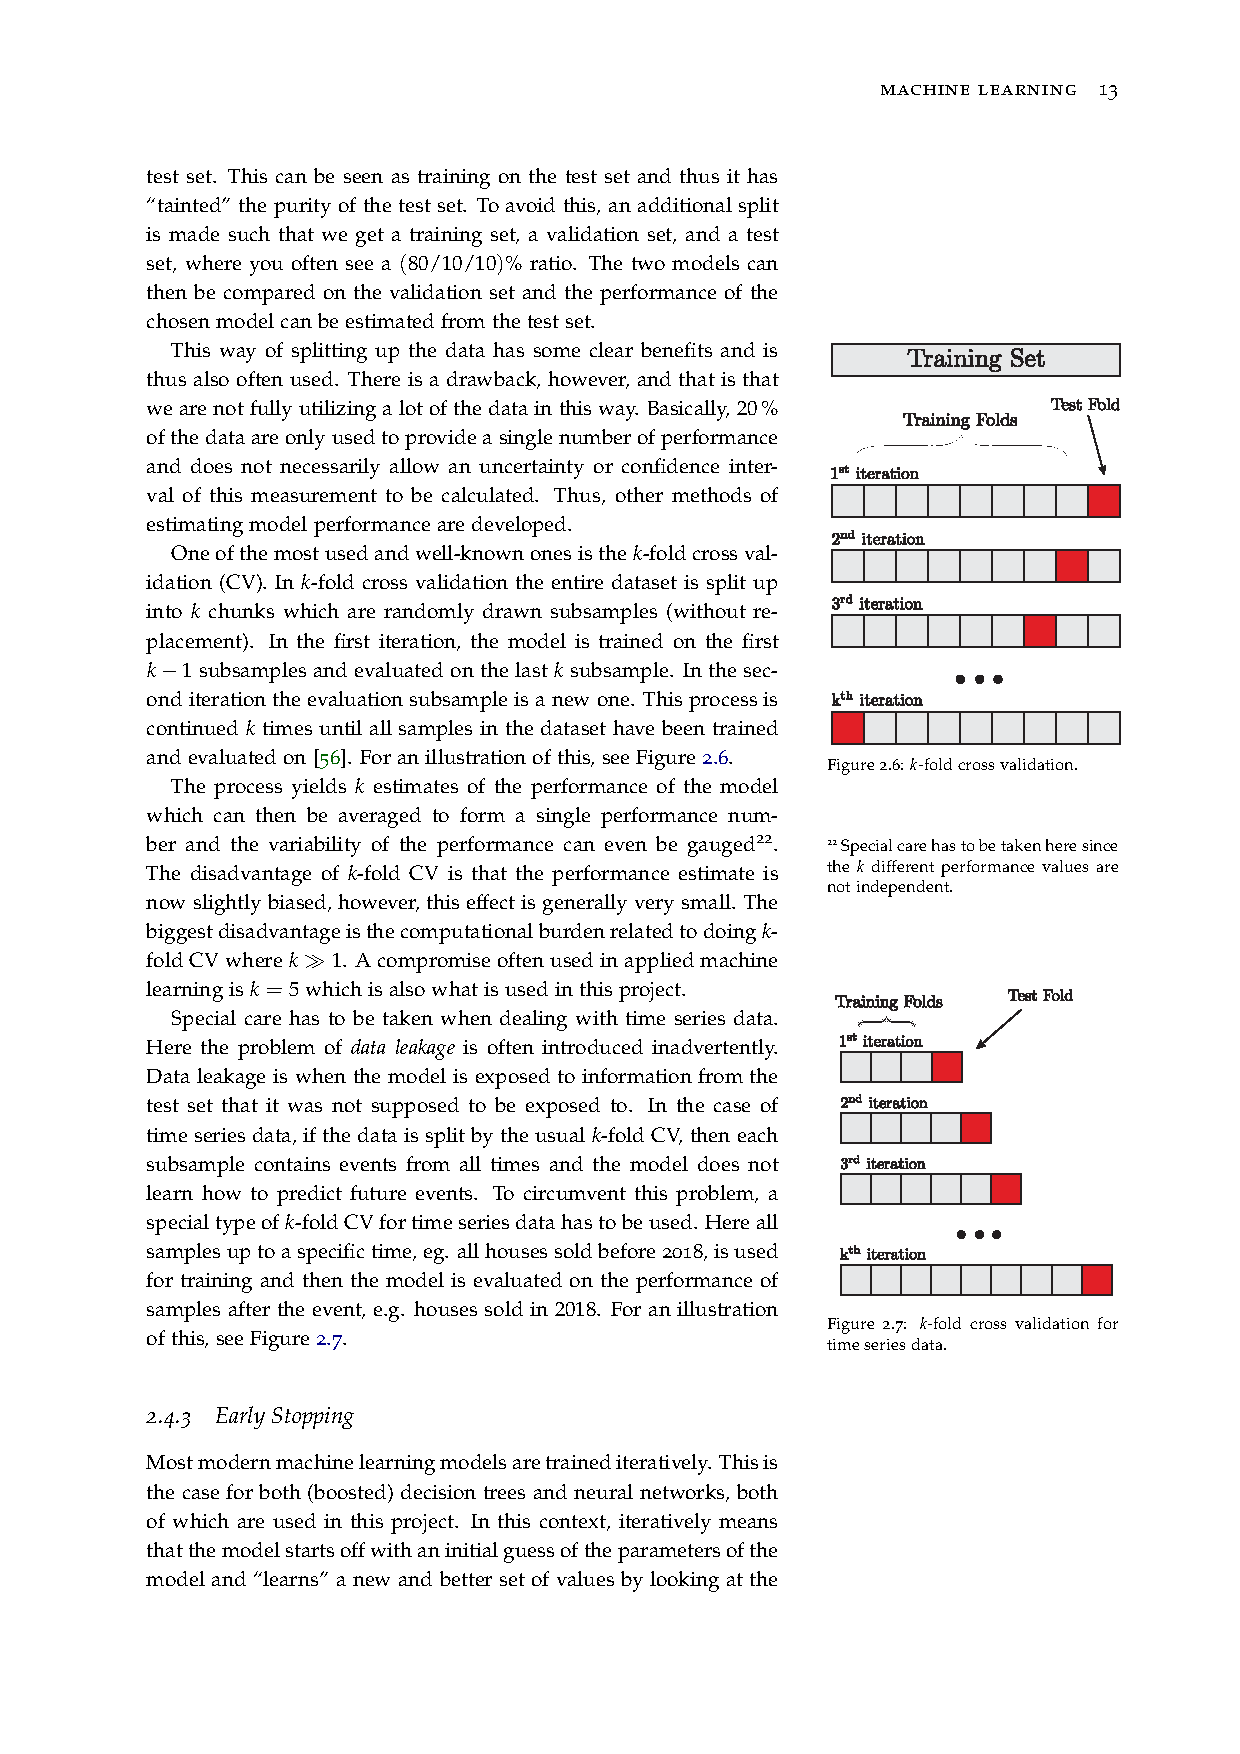
\includegraphics[trim={14cm 17cm 1.95cm 6.5cm}, clip, width=.8\linewidth]{figures/MasterThesis-cross-validation}
        \caption{$K$-fold cross validation}
        \label{fig:ML-crossval-kfold}
    \end{subfigure}%
    \begin{subfigure}{.5\textwidth}
        \centering
        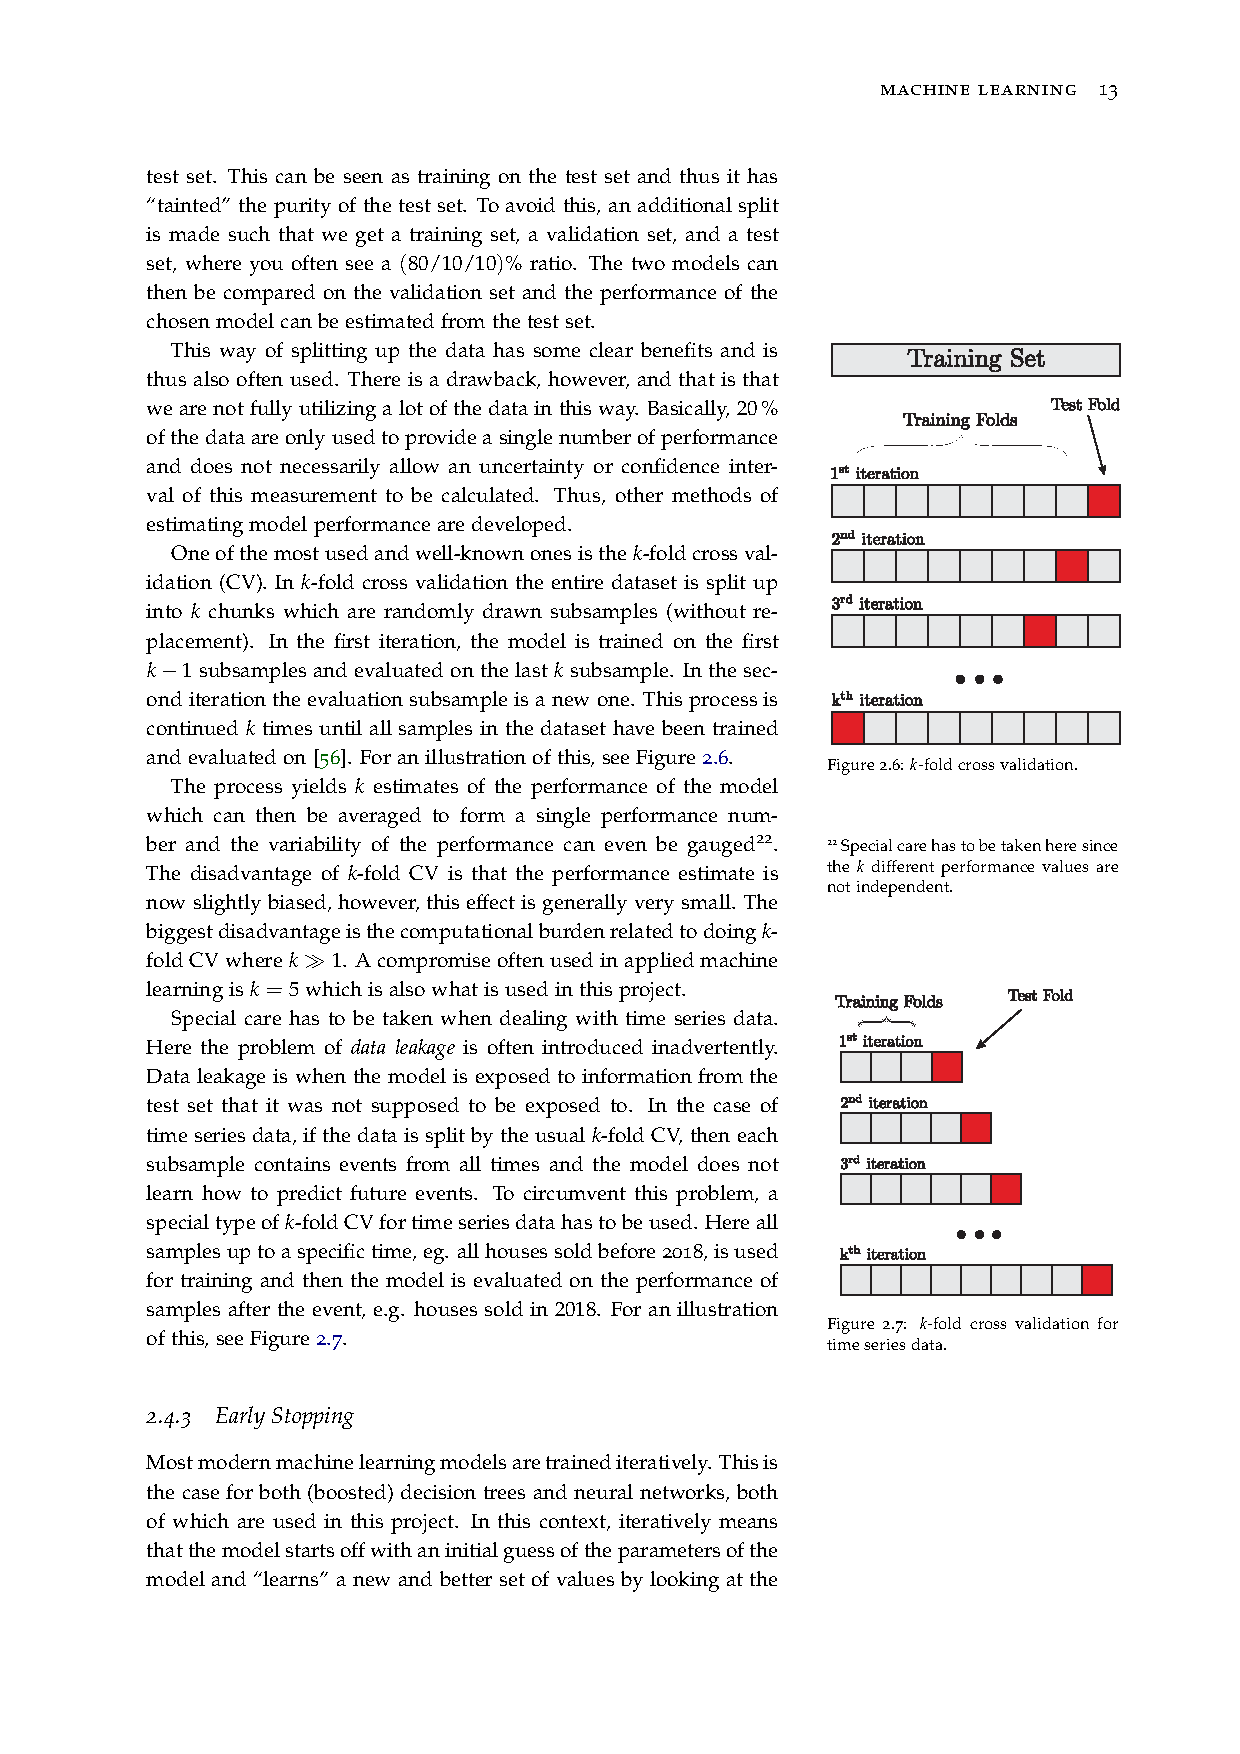
\includegraphics[trim={14.14cm 7.67cm 2.1cm 16.5cm}, clip, width=.8\linewidth]{figures/MasterThesis-cross-validation}
        \caption{Temporal cross validation}
        \label{fig:ML-crossval-temporal}
    \end{subfigure}
\end{figure}

The actual training of the learning model $\mathcal{A}$ is model-dependent and will not be covered in this thesis. The term training refers of the optimization of the internal parameters in the ML model. In most cases, the training depends on the gradient of the loss function with respect to internal parameters to be computed, see \cite{michelsenPhysicistApproachMachine2020} for a more detailed description of the training process.

Training is not the only way to optimize the performance of  $\mathcal{A}$, albeit it is the primary one. In addition to the internal parameters of the model, some parameters are external to the model in the sense that they are not optimized by the model itself, but rather by the user. These are called hyperparameters and are often optimized using a technique called hyperparameter optimization (HPO). In the case of logistic regression, the number of variables to include would be an example of a hyperparameter; in the case of a decision tree model, the depth of the tree. Hyperparameter optimization can be performed in many ways, where the common one is through grid search, see \autoref{fig:ML-hpo-GS}.
\marginfig{figures/MasterThesis-hpo-grid.pdf}{Illustration of grid search. Figure from \cite{michelsenPhysicistApproachMachine2020}.}{fig:ML-hpo-GS}

In grid search, all combinations of the hyperparameters (the cartesian product) are tested and the best combination is chosen. This is a simple and intuitive approach, however, it scales exponentially with the number of hyperparameters. As such, grid search suffers from the curse of dimensionality. In addition to this, it depends on the user-defined grid, which might not be optimal. To circumvent this, a technique called random search (RS) was developed \autocite{bergstraRandomSearchHyperparameter2012a}. Random search is a randomized version of grid search, where the hyperparameters are sampled randomly from a distribution. This allows for a more efficient sampling of the hyperparameter space, see \autoref{fig:ML-hpo-RS}. Another advantage is that RS lets the user decide on the number of iterations beforehand.

\begin{figure}[htbp]
    \sidecaption{
        Illustration comparing grid search to random seach. The height of green surve is the score-function which has to be optimized. Figure from \cite{bergstraRandomSearchHyperparameter2012a}.
        \label{fig:ML-hpo-RS}}
    \centering
    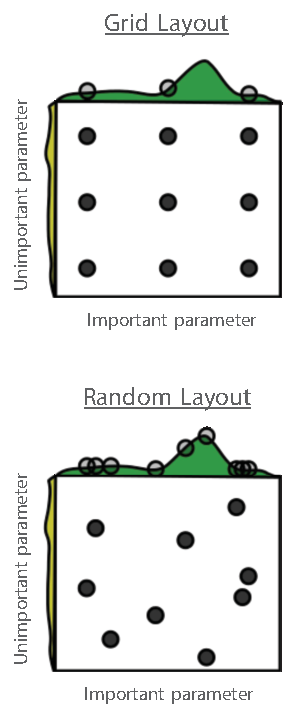
\includegraphics[trim={5.7cm 20cm 5.7cm 3cm}, clip, width=.8\linewidth]{figures/MasterThesis-hpo-random}
\end{figure}

The disadvantage of random search is that all draws are fully independent. While this allows for easy parallelisation of the algorithm, this also means that each new sample might be infinitesimal close in the hyperparameter space to a previous sample with bad performance, which with high probability will thus also have a high loss. An approach that does take the history of the previous samples' performance into consideration is Bayesian optimization \autocite{brochuTutorialBayesianOptimization2010a}. In Bayesian optimization each successive hyperparameter is chosen based on an acquisition function, which optimizes the expected improvement in the performance of the model. This is illustrated in \autoref{fig:ML-hpo-BO}. This leaves the user with the task of choosing between ``exploitation'' and ``exploration'' of the hyperparameter space in the definition of the acquisition function, yet most implementations of bayesian optimization have decent default settings.

\begin{figure}[htbp]
    \sidecaption{
        Illustration of the learning process of Bayesian optimization. The previous observations are shown as black dots and the true objective function is shown as a dashed black line. This line is fitted with Gaussian processes which is shown as the solid line with its uncertainty in purple. The acquisition function is shown in green and its maximum decides what the next iteration of the hyperparameter value(s) should be \autocite{michelsenPhysicistApproachMachine2020}.
        \label{fig:ML-hpo-BO}}
    \centering
    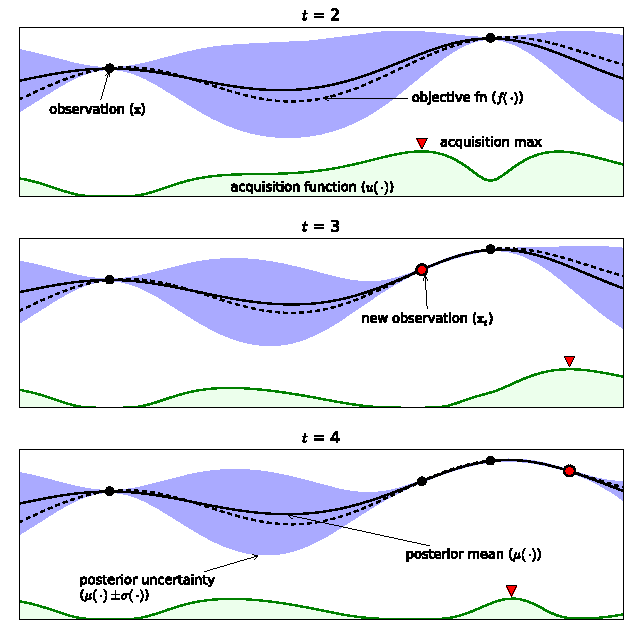
\includegraphics[width=0.8\textwidth]{figures/MasterThesis-hpo-bayesian}
\end{figure}

We use the Python package Optuna \autocite{akibaOptunaNextgenerationHyperparameter2019} for HPO in Paper II due to its ease of use and its support for Bayesian optimization. In particular, we use the Tree-structured Parzen Estimator algorithm for the Bayesian optimization and a median stopping rule to minimize optimization time \autocite{bergstraAlgorithmsHyperParameterOptimization2011}. This allowed for a good comporise between optimization time and performance.

While model performance is often paramount, in some fields -- such as medicine -- being able to explain the model's predictions is almost as important. This is especially true in the case of medical decision support systems, where the model is used to make decisions about the patient's treatment. Model explainability helps to build trust in the model, for both the patient and the medical staff alike.

In Paper II, we employ the SHapley Additive exPlanations (SHAP) values which provide estimates on which variables contribute most to the risk score predictions \autocite{lundbergUnifiedApproachInterpreting2017,lundbergLocalExplanationsGlobal2020}. SHAP values allow for not only a global explanation of the model, i.e. which features are most important generally, but also a local explanation, i.e. which features led to a single patient being predicted at risk of being re-hospitalized. It has previously been shown that the interaction between SHAP values and medical doctors can improve the performance of anaesthesiologists \autocite{lundbergExplainableMachinelearningPredictions2018a}.

While the aim of Paper II is to show how modern machine learning techniques can be used to improve the risk prediction process, the usefulness of the SHAP values in a medical context is demonstrated in our paper in \autoref{appendix:anaemia}. The paper uses the SHAP values to compare the preoperative haemoglobin level in the patient with the risk-score, stratified by sex and operation type (knee vs. hip replacement). Currently, the WHO guidelines for the haemoglobin levels are gender specific, however, our study finds no significant gender difference and a haemoglobin threshold close to the WHO suggestions for men \autocite{anaemiasNutritionalAnaemiasReport1968}.